%parler des lib quand on s'en sert
%parler des standby liste

%à faire aussi le schéma UML


% \newpage et \noindent inutiles
% On est pas sensé se soucier de la mise en page...
% Si tu veux une nouvelle page après chaque paragraphe, tu insert pas 130
% \newline, tu fais une seule règle en haut du fichier qui précise "Sauter une
% page après chaque paragraphe"




\documentclass[a4paper, 12pt]{report}

\usepackage[utf8]{inputenc}
\usepackage[francais]{babel}
\usepackage{graphicx}
\usepackage{bookman}
\usepackage{titlesec}
\titleformat{\chapter}[hang]{\bf\huge}{\thechapter}{2pc}{}
\renewcommand\thesection{\Roman{section}}
\renewcommand\thechapter{\Roman{chapter}}

\title{Rapport Manic Shooter}
\author{Adrien \bsc{Boutigny}, Tanel \bsc{Creusier} et Matthieu \bsc{Dechipre}}
\date{L2 Informatique 2015--2016}

\pagestyle{headings}

\begin{document}

\maketitle

\tableofcontents

\chapter{Introduction}
	\section{Contexte}
Le shooter est un domaine très vaste du jeu vidéo utilisant des codes et des
logiques bien à lui. Lors de ce semestre, nous avons dû travailler sur un
sous-genre de jeu de tir, le Manic Shooter. Ce type de jeu impose plusieurs
choses, tout d'abord, un nombre de projectiles ahurissant et en règle général
une dextérité importante de la part du joueur pour ce mouvoir dans ce maelström
de balles, de tirs et de lasers en tout genre.

Ci-dessous, voici l'un des piliers du genre, DoDonPachi:

\begin{figure}[!ht]
\centering
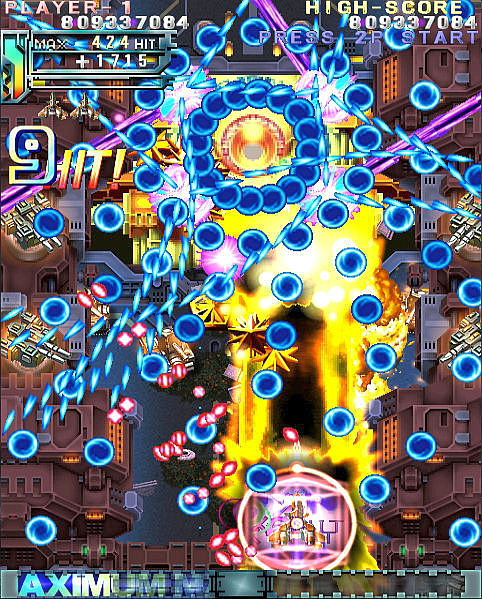
\includegraphics[scale= 0.4]{images/dodonpachi.jpg}
\caption{DoDonPachi}
\end{figure}

    \section{Objectifs du projet}
Dans cette application que, il faut que le joueur
puisse passer aux commandes d'un vaisseau capable de se déplacer, de tirer et
d'utiliser divers bonus et items récupérables au cours de la partie. \newline

\noindent De plus, il faut également gérer les ennemis. Etudier des manières de
se déplacer, de tirer pour ces derniers. Il faut aussi réfléchir aux méthodes
d'apparition possibles et trouver comment faire en sorte que les projectiles
tirés par le joueur touchent les vaisseaux ennemis et leurs fassent perdre des
points de vie.\newline

\noindent L'idée est donc de créer un jeu de tir utilisant le clavier pour les
déplacement, dans un premier temps, et le tir via une librairie python prévu
spécialement pour  tout ce qui est multimédia (événementiel, vidéo \ldots) Dans
un second, il faut peut-être imaginer une manière plus dynamique de déplacer
le vaisseau du joueur, pour ce type de shooter, la précision est de rigueur.
Aussi faut-il permettre au joueur de modifier soi-même ses touches dans un
second temps. \newline

\noindent Le premier semestre s'est vu consacré à la création des fonctions
principales du programme, comme le déplacement, l'affichage des vaisseaux
\ldots Dans une première partie, nous expliquerons donc ce que nous avons
décidé de mettre en place pour ce jeu, toutes les fonctionnalités que nous
avons prévu
d'implémenter.

\chapter{Cahier des charges}
    \section{Fonctionnalités à réaliser}
Pour nous lancer dans la création ce Manic Shooter, nous avons commencé par
faire un brain storming pour déterminer tout ce dont nous avons besoin pour
faire ce jeu et ce que nous devons implémenter. Ainsi, nous avons obtenu les
fonctionnalités suivantes: \newline

\begin{itemize}
    \item un vaisseau joueur pouvant tirer et se déplacer
    \item un système de score
    \item un menu
    \item un système de musique
    \item différents types d'ennemis eux aussi capables de se déplacer et de tirer
    \item gestion des collisions entre les ennemis, les projectiles et le joueur
    \item des powers-ups
    \item un menu et un système de configuration des touches
    \item un système de génération de niveaux
    \item des décors
\end{itemize}

\noindent Nous essaierons d'implémenter toutes les fonctionnalités ci-dessus
tout le long de cette année en effectuant la partie principal du travail
pendant le premier semestre. Lors du second, nous implémenterons tous les
éléments qui n'auront pas été implémenté pendant le premier semestre. Ensuite,
si nous atteignons nos objectifs, nous implémenterons des fonctionnalité
supplémentaires et nous optimiserons le programme afin qu'il soit plus
performant.

\chapter{Fonctionnement}
	\section{Interfaces}

Pour créer ce shooter, nous commençons par créer une fenêtre afin d'y afficher
tout ce dont nous avons besoin. Pour ce faire, nous utilisons Pysdl2. Pysdl2
est une librairie utilisée pour créer des applications multimédias en deux
dimensions. Elle nous fournit donc un accès bas niveau aux sorties vidéos,
audio, au clavier et à la souris de notre machine (également aux manettes mais
nous n'avons pas prévu de gérer ceci). Nous utilisons cette librairie sous
Python 3.4. \newline

\noindent Cette nouvelle fenêtre est l'interface du jeu. Celle-ci affiche tous
les ennemis actifs du jeu, le joueur, les projectiles actifs (amis et ennemis)
en utilisant les fonctions de la librairie Pysdl2. Cette interface communique
avec un objet monde que nous créons au lancement du programme et qui contient
certaines informations importantes pour le déroulement du jeu. Entre autres,
nous pouvons citer la caméra qui nous permet de gérer le scrolling vertical de
notre jeu. \newline

\noindent Cette ``caméra''  est créée également à l'initialisation du jeu et se
déplace constamment vers le haut en faisant défiler le fond du jeu. Les
coordonnées en y de la caméra ne font donc que diminuer (on se situe dans un
repère inversé). La carte est pré-établie au lancement du niveau, les ennemis
aussi. En remontant, on va donc vérifier si les coordonnées en y des ennemis
coïncident avec celles de la caméra grâce à notre fonction de collision (cf ci
après). Si la caméra entre en collision avec les vaisseaux ennemis contenus
dans une liste créée au tout début du programme alors on les active et on les
affiche.\newline

\begin{figure}[!ht]
\centering
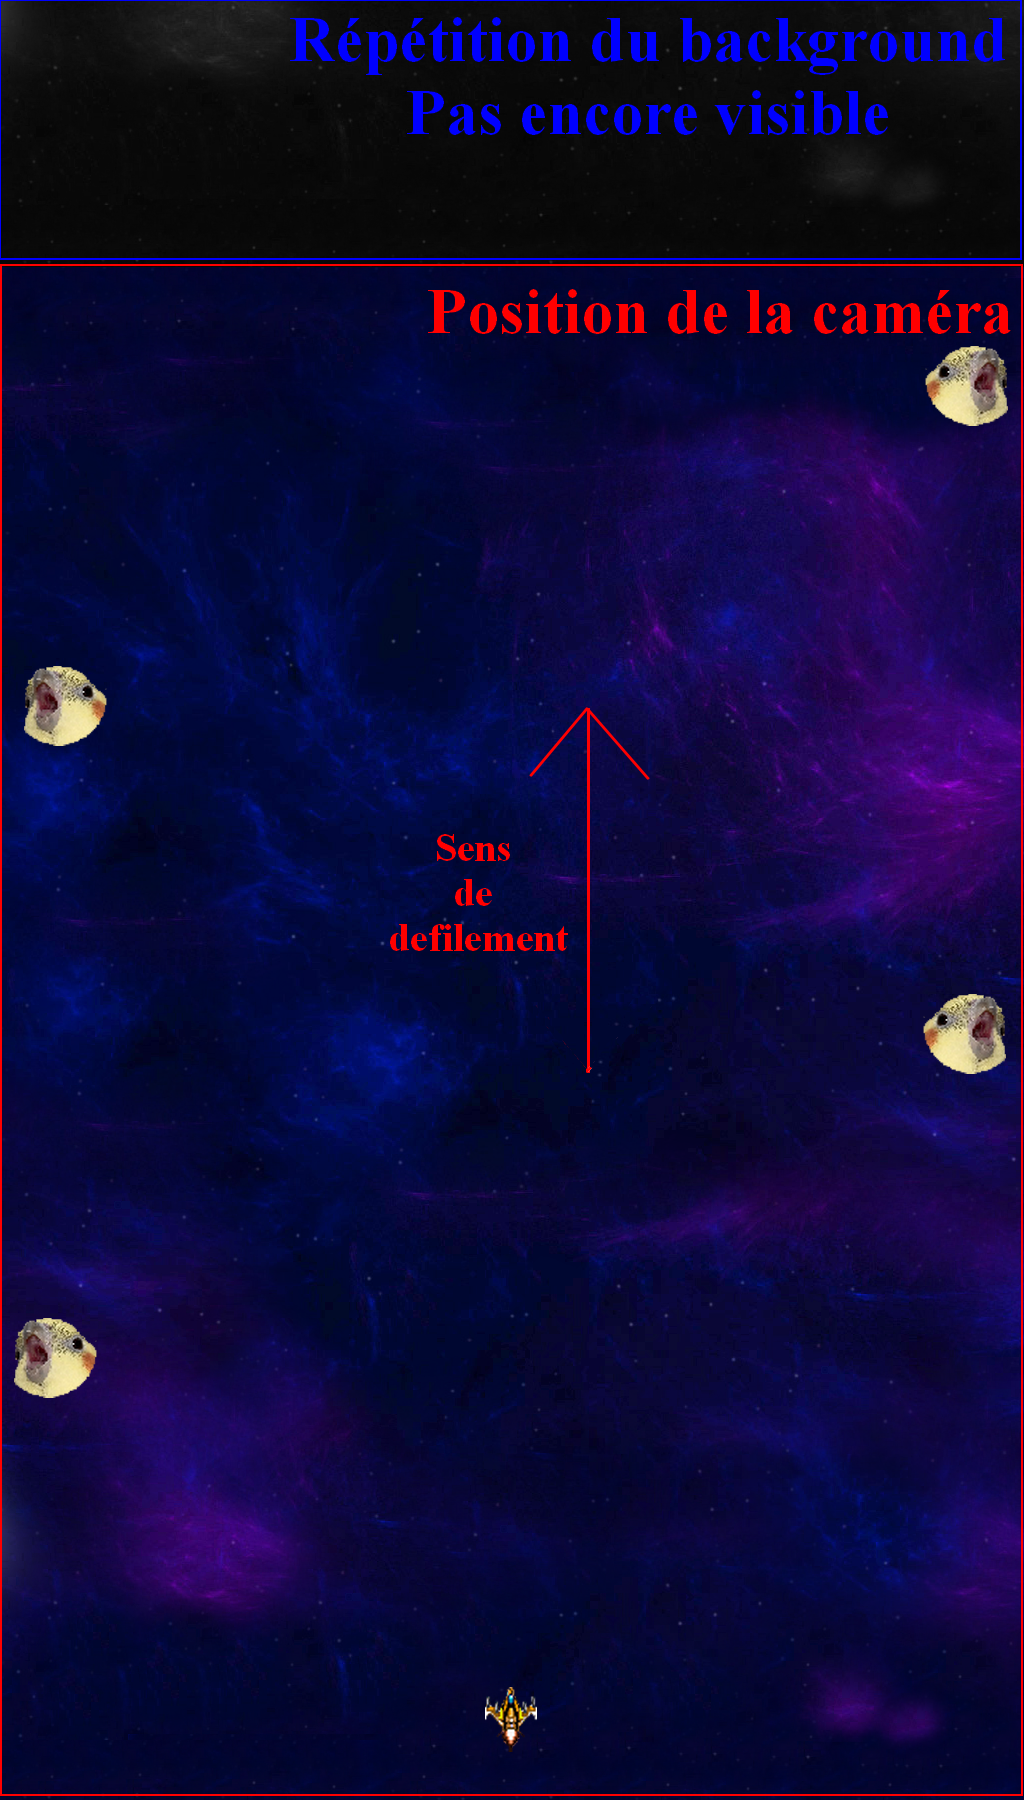
\includegraphics[scale= 0.4]{images/schema.png}
\caption{Principe de la caméra}
\end{figure}

\noindent Le monde contient également le vaisseau du joueur qui doit être
manipulé par l'utilisateur et qui peut dans cette première version tirer et
bouger. Comme dit précédemment, les ennemis actifs et passifs (ceux qui ne sont
pas encore arrivés à l'écran) sont contenus dans le monde, ainsi que tous les
projectiles qui ont été tiré. \newline

\noindent Les méthodes des vaisseaux ennemis et du joueur interagissent donc
avec le monde et ce qu'il contient lors des collisions par exemple ou encore
lorsqu'ils tirent.

%\subsection{Pyglet}
%
%Nous avons utilisé Pyglet simplement pour permettre de gérer le flux
%audio, ce que la librairie pysdl2 ne permet pas nativement, en tout cas pas
%sans un travail de fond. Aussi, nous avons trouvé une solution temporaire via
%Pyglet pour ajouter une ambiance sonore au jeu.\newline
%
%\noindent Cette librairie est, tout comme Pysdl2, une librairie multimédia qui fait
%quasiment le même travail que cette dernière. Aussi, elle est trop volumineuse
%pour une simple librairie audio. Aussi, nous espérons faire en sorte de faire
%fonctionner la librairie audio de Pysdl2 le long du second semestre et ainsi
%remplacer Pyglet.
%
%\noindent Des exemples de fonctionnement de la partie audio de SDL sont déjà disponibles
%sur le dépot.

\section{Vaisseaux}

Nous avons implémenté les vaisseaux de manière à ce qu'il se base tout
sur un modèle commun. Ce modèle commun définit des paramètres par défaut d'un
vaisseau quelconque, les points qu'il attribue au joueur lorsqu'il est détruit
ou ses points de vie par exemple.\newline

\noindent A partir de ce squelette de vaisseau, nous avons créé des sous
classes pour tout les autres vaisseaux, celui du joueur d'un côté, avec ses
méthodes propres, et ceux des ennemis de l'autre. Chaque ennemi a ses méthodes
et chaque ennemi est spécifique. Certains se contenteront de passer sans rien
faire, d'autres pourront tirer en visant le joueur ou d'autres encore pourront
se déplacer en suivant un chemin complexe (cercle, sinusoïde \ldots)\newline

\begin{figure}[!ht]
	\centering
	\begin{minipage}[t]{.49\linewidth}
		\centering
		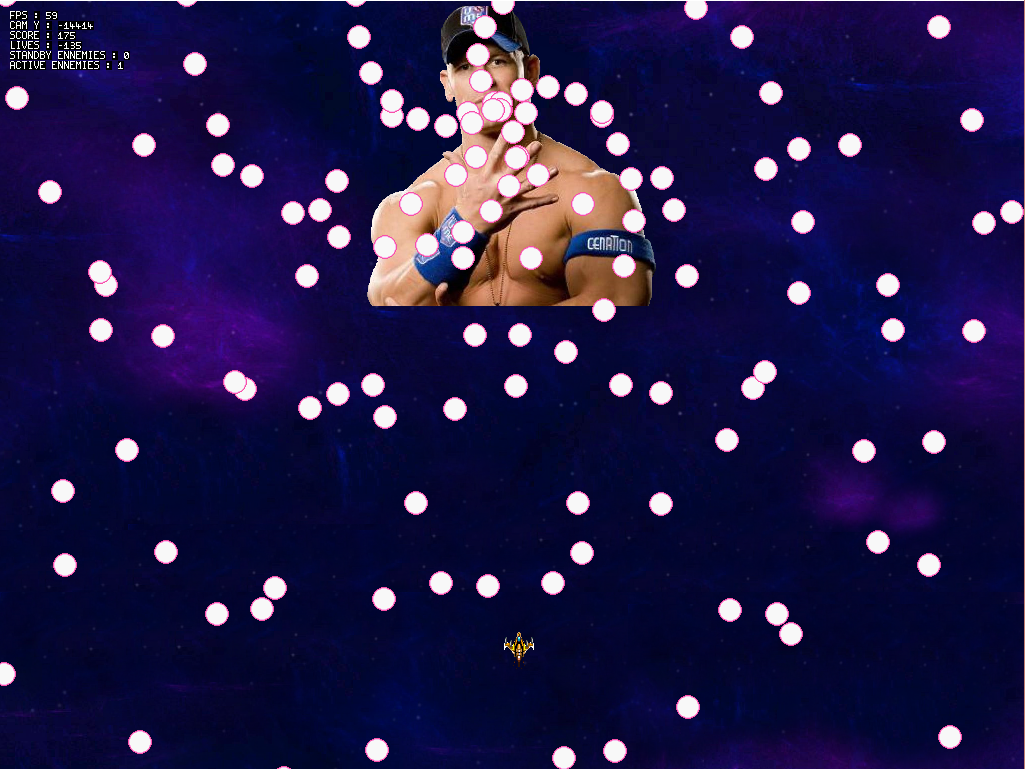
\includegraphics[height=200pt, width=180pt]{images/johncena.png}
		\caption{Ennemi tirant beaucoup de projectiles}
	\end{minipage}
	\begin{minipage}[t]{.49\linewidth}
		\centering
		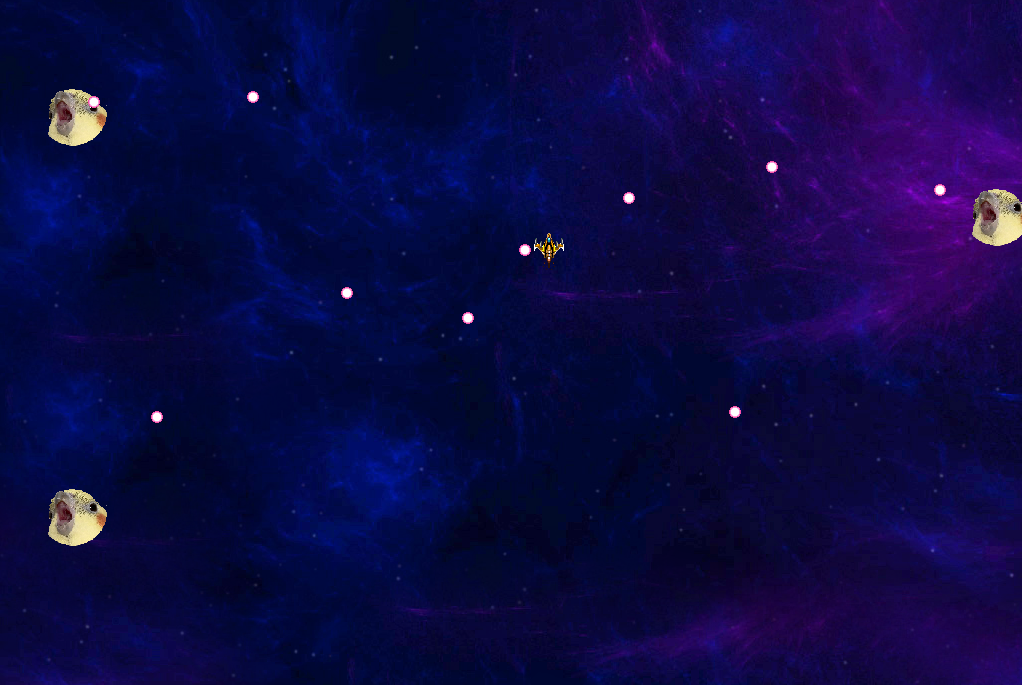
\includegraphics[height=200pt, width=180pt]{images/poissons.png}
		\caption{Ennemis visant le joueur}
	\end{minipage}
\end{figure}

\noindent De ce fait, nous avons un module plutôt conséquent contenant tous les
types de vaisseaux différents. Dans le jeu, on doit savoir si un vaisseau entre
en collision avec un autre vaisseau ou encore si un vaisseau entre en collision
avec un projectile, il faut donc détecter pour chaque vaisseau présent sur
l'interface s'il entre en collision avec un autre élément (vaisseau du joueur
dans le cas d'un vaisseau ennemi, vaisseau ennemi dans le cas contraire et
projectiles).

\section{Collisions}

\noindent Les collisions sont au coeur de notre projets. Et bien que la
gestion de celles-ci soit d'une simplicité enfantine, elle n'en demeure pas
moins utilisée par quasiment tout les modules, et en très grand nombre.

Pour la gestion des collisions, on a le choix entre 2 méthodes différentes
ayant chacune ses avantages et ses défauts:
\begin{itemize}
    \item Soit on utilise des formes géomètriques (des rectangles) et on teste les collisions
        en vérifiant des inéquations ``simples''. Méthode simple à mettre en
        place et rapide.
    \item Soit on utilise des ``masques de collisions'', c'est à dire une image
        ``invisible'' qui sera superposée à l'element concerné. L'image suit un
        code couleur indiquant quelles sont les parties solides de l'element.
        Par exemple, un pixel blanc indique que l'element est solide et un
        pixel noir qu'il n'y a rien à cet endroit. Pour savoir si deux élements
        rentrent en collision, on teste si des pixels ``blancs'' se
        superposent.
\end{itemize}

Pour l'instant nous utilisont uniquement des collisions à base de rectangles.
Le coût peu élevé de l'algorithme nous arrange car nous avons parfois des
centaines de collisions à tester à chaque frame.

%inserer une image d'un vaisseau ennemi avec un rectangle representant sa
%hitbox, qu'on voit bien que la hitbox couvre pas forcement tout le sprite

\noindent Cet algorithme peut s'exprimer facilement avec l'illustration tirée du
site développez.com suivante. Ici, le bleu est avant la ligne jaune minimum du
rouge, bleu et rouge ne sont pas en collision et le jaune est avant le maximum
du rouge, ils sont en collision:

\begin{figure}[!ht]
\centering
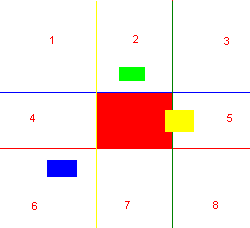
\includegraphics[scale= 0.8]{images/collision-boites.png}
\caption{Principe de collisions simples}
\end{figure}

\newpage

\section{Génération des vagues}

%à faire
%parler des standby, active etc ...

La classe World encapsule entre autre deux listes de vaisseaux ennemis (des
objets EnnemyShip). Ces deux listes sont \verb|standby_ennemies| et
\verb|active_ennemies|.
Cette séparation en deux liste permet d'optimiser le temps de calcul utilisé
pour traiter les ennemis du niveau.

Pour l'instant, on génère les niveaux ``à l'avance''. Grâce à l'utilisation des
deux listes citée, avoir plusieurs milliers d'ennemis pré-généré n'aura pas
plus d'impact en terme de performance qu'une dizaine d'ennemis.

\subsection{standby\_ennemies}

La première contient les ennemis inactifs du niveau, c'est à dire ceux qui ne
sont pas encore apparu à l'écran. Le contenu de cette liste est generé
\emph{avant} le début du niveau.

A chaque frame, on parcourt cette liste afin
de determiner quels sont les ennemis à \emph{activer}. Aucune autre opération
n'est effectuée sur ces objets, ce qui permet d'économiser des ressources.

Lorsqu'un ennemi est \emph{activé}, on le supprime de la liste
\verb|standby_ennemies| et on l'ajoute à \verb|active_ennemies|.

De plus, cette liste est utilisée comme une pile dans laquelle la tête sera
toujours le prochain ennemis à apparaitre (les objets sont trié par position
Y). Ainsi, dès que l'on tombe sur un vaisseaux qui n'a pas à apparaitre à
l'écran, on arrête de parcourir la liste.

\subsection{active\_ennemies}

Cette liste contient les ennemis présents à l'écran. Pour chacun d'eux, il faut
tester plusieurs choses:
\begin{itemize}
    \item Les collisions avec un laser tiré par le joueur.
    \item Sa ``mise à jour'' (déplacement, tir de boulette, etc)
    \item S'il faut le retirer de la liste pour une raison quelconque (sorti de
        l'écran, détruit par le joueur, \ldots)
\end{itemize}

\chapter{Réalisation}
\section{Répartition des tâches}

Après avoir fait la liste de tout ce dont nous avions besoin pour créer ce jeu,
nous avons réparti les tâches entre les différents membres du groupe. Chacun
s'est lancé dans ce qu'il voulait faire. En effet, nous pouvions développer
chacun de notre côté assez facilement. Nous avons pu implémenter simultanément
la boucle principale gérant le jeu, le système de collisions et les différents
vaisseaux.\newline

\noindent Par la suite, il est facile de travailler sur les modules externes
comme les bonus, le système de configuration des touches ou encore d'autres
types d'ennemis et ensuite les greffer au code déjà existant.

\chapter{Retours sur l'application et apports possibles}

Nous avons pu implémenté pour l'instant une bonne partie des éléments du
projet, à savoir des vaisseaux différents, un vaisseau joueur pouvant tirer et
se mouvoir. Nous avons également mis en place un menu de départ qui reste
encore à fignoler et le système de collisions. Nous avons également la
possibilité de mettre en pause le jeu. \newline

\noindent Les ennemis ont quelques patterns de mouvements et de tirs originaux
mais pour l'instant nous n'avons pas de choses vraiment complexes comme des
laser continus ou encore des boucliers. Nous essaierons donc de mettre ces
éléments en place lors du second semestre ainsi que le générateur de niveaux et
la possibilité de modifier sa configuration de contrôle. \newline

\noindent Nous mettrons aussi en place divers bonus parmi ceux cités
précédemment comme des laser continu, des boucliers, des accélérations de tir
ou encore des explosions à courte portée. Il faudra également remplacer la
gestion du son de la librairie Pyglet par la partie audio de SDL\@.

\chapter{Suppléments}
	\section{Sources}
https://www.libsdl.org/
https://www.python.org/download/releases/3.4.0/ \newline
https://bitbucket.org/pyglet/pyglet/wiki/Home

	\section{Documentation}
\noindent http://www.developpez.com/ \newline
https://openclassrooms.com/ \newline
https://pysdl2.readthedocs.org/en/latest/ \newline
https://pyglet.readthedocs.org/en/pyglet-1.2-maintenance/

\end{document}
